\section{Experimental Setting}
\label{sec:experimental-setting}
The goal of this evaluation is to show how \name can extend the traditional hypothesis based research towards the Systematic Comparative Research approach. First of all we have to define the experimental setting of the evaluation. In Chapter \ref{chap:heaven} we define an experiment as the tuple $<\mathcal{D}, \mathcal{T},\mathcal{E}, \mathcal{Q}>$, where:
\begin{itemize}
\item $\mathcal{E}$ is the RSP Engine
\item $\mathcal{D}$ is the Dataset 
\item $\mathcal{T}$ is the Ontology
\item $\mathcal{Q}$ is the Query that $\mathcal{E}$ continuously answers.
\end{itemize}

The experimental setting must include different tests to cover the most important variations on the tuple above. 

The Baselines (see Section \ref{sec:baseline} and Section \ref{baseline-impl}) are the RSP Engines subject of our experiment, $\mathcal{E}$.  The purpose of these tests is to show how difficult is attempting to prove even simple hypothesis formulated starting from the knowledge of the RSP Engine model, and consequently why we need \namens . Top-Down investigations are in general not easy for commercial solutions like C-SPARQL Engine and CQELS, because the complexity of their architecture is too high to be easily faced in order formulate hypothesis of comparison.  For the baselines instead this survey is possible, because we have a complete model of their system, SERE properties clarify how to develop the investigation and last but not least we know many implementation details that can help during the analysis. Chapter \ref{chap:heaven} shows how the four implementations of the baselines differ most for two characteristics, RDF Stream Model and Reasoning architecture. The following table summarises these few but well defined differences, naming the four baselines for the evaluation:\begin{table}[htb]
\scriptsize
\centering
\begin{tabular}{c|cc} % creating eight columns
	\hline
         & Naive & Incremental\\
	\hline
	Graph        &  B1      & B2\\
	Statment   &  B3   & B4\\
	\hline % inserts single-
\end{tabular}
\caption{Configuration of the four baselines}
\label{tab:baselines-names}
\end{table}

\noindent Formulating simple hypothesis of comparison about which approach is better then an other one is simple among these four configurations. In Chapter \ref{chap:problem-setting} we describe which requirements guarantee that an RSP Engine is a baselines (SERE properties): Simplicity, Elementarily, Relevance and Eligibility allow us to evaluate the baselines as a simple term of comparison for further research on Stream Reasoning systems. %qui voglio dire che la valutazione delle baseline ha un suo senso dato da queste proprpiet�, lo sappiamo ma non lo indaghiamo ora con quello scopo.
Finally, wow we realised the baselines is described in Chapter \ref{chap:implementation-experience}; the know-how about their internal mechanisms may help in the data analysis motivating behaviours which are unpredictable form the architectural viewpoint. 

Te Dataset  $\mathcal{D}$ and the Ontology $\mathcal{T}$ must be chose to ensure the baselines Simplicity, as stated in Section \ref{sec:baselines}. We take $\rho$DF  \cite{DBLP:conf/esws/MunozPG07}  as their entailment regime, because several works in the field  \cite{DBLP:conf/semweb/UrbaniMJHB13}  choose this as the minimal meaningful task for a Stream Reasoner. In particular, $\rho$DF is the RDF-S fragment that reduce complexity while preserving the normative semantics and core functionalities. The RDF streams  $\mathcal{D}$ used in the experiments are obtained streaming in different ways the data generated with LUBM  \cite{Guo2005} and the ontology $\mathcal{T}$ is the LUBM one\footnote{http://swat.cse.lehigh.edu/onto/univ-bench.owl}. We assume that the ontology does not change over time, therefore the materialisation of $\mathcal{T}$ is computed before starting the experiment and the RSP engine does not have to perform this task. It is worth to discuss the choice of using data from LUBM over SRbench and LSbench. The first one has data, which are not adequate for the experiments, since they do not require any reasoning. The SRbench data, on the contrary, requires reasoning, but, being real-data, do not have the possibility to be scaled up and down. This choice accomunate us to previous works on Stream Reasoning \cite{DBLP:conf/semweb/UrbaniMJHB13}. The data generator system, responsible to build $\mathcal{D}$ w.r.t. $\mathcal{T}$, is able to scale both in terms of dimension of the dataset and the reasoning effort. Being LUBM static data, we exploit the \textsc{RDF2RDFStream} component of the test stand that takes care to adapt the data generate by LUBM to a streaming scenario. The component can be set up to obtain an RDFStream where the number of triples with the same timestamps follows a given discrete function, Section \ref{sec:streamer-impl} contains the implementation details of this particular \textsc{Streamer}. %e' veramente il timestamp quello?

The experiments in this Section are thought to show what kind of testing is possible trough \namens. We designed two kind of experiments based on the \textsc{RDF2RDFStream} capabilities of controlling the triple distribution in the RDFStream to evidence system dynamics over a particular input. Both the experiment typologies belong to the category of Stress Test:
\begin{itemize}
\item \textbf{SOAK}: the number of contemporary triple in the RDFStream does not change during the experiment.
\item \textbf{Step Response} the number of contemporary triple suddenly changes during the experiment, usually increasing of a degree of magnitude.
\end{itemize}
 


Finally, the queries $\mathcal{Q}$, used in the experiments, are variants of the same two basic identity queries that continuously asks for the materialisation of the current window:
\begin{enumerate}
\item[Q.1]  Naive
\item[Q.2] Incremental
\end{enumerate}
 		 
Q.1 outputs the snapshot of the entire window and it is used for the Naive reasoning approach; Q.2 outputs the ir-streams and it is used for the Incremental reasoning approach. The queries differ for the size $\omega$ of the sliding window. In particular, we use windows in which $\omega$ is an integer multiple of the slide parameter $\beta$ of the window, i.e., it holds that $\omega = \beta * N$. In other words, $N$ is the number of \textsc{CTEvents} that the window can contain. 

Moreover, Section \ref{sec:baselines-impl} shows how the proposed baselines take advantage of the ability of Esper to be temporally controlled by an external agent\footnote{\url{http://esper.sourceforge.net/esper-0.7.5/doc/reference/en/html_single/index.html#api-controlling-time}} by sending time-keeping events to synchronise the internal time flow. One time-keeping event is sent before injecting the triples in a \textsc{TCEvent} and another one after all triples in \textsc{TCEvent} were sent. In this way all the triples in the \textsc{TCEvent} are consider contemporary by the baselines and each TCEvent can be seen as a proxy for the timing event. Together with the RDF2RDFStream is possible to estimate the content of the current window in terms of number of RDF Triples in any moment of the experiment.\\

Following we describe in details the content of the SOAK (Section \ref{sec:soak-es}) and the Step Response tests (Section \ref{sec:step-es}), providing a lecture key for the results presented in the last part of this Chapter.

\section{Experiment Design}

The goal of this Chapter is to show how \name can improve the top-down analysis method. Traditionally, the deep comprehension of a theoretical problem together with the knowledge of the model, maybe supported by the implementation experience, allow to formulate hypothesis of the system behaviour. Experiment design starts with some assumptions about the system, for example in Section \ref{sec:experimental-setting} we explain the reasons why we chose $\rho$DF as entailment regime for our experiments. Researchers formulate hypothesis on the base of these assumption, and they design experiments to verify hypothesis validity. Figure \ref{fig:experiment-design} summarises this approach.

\begin{figure}[tbh]
  \centering
	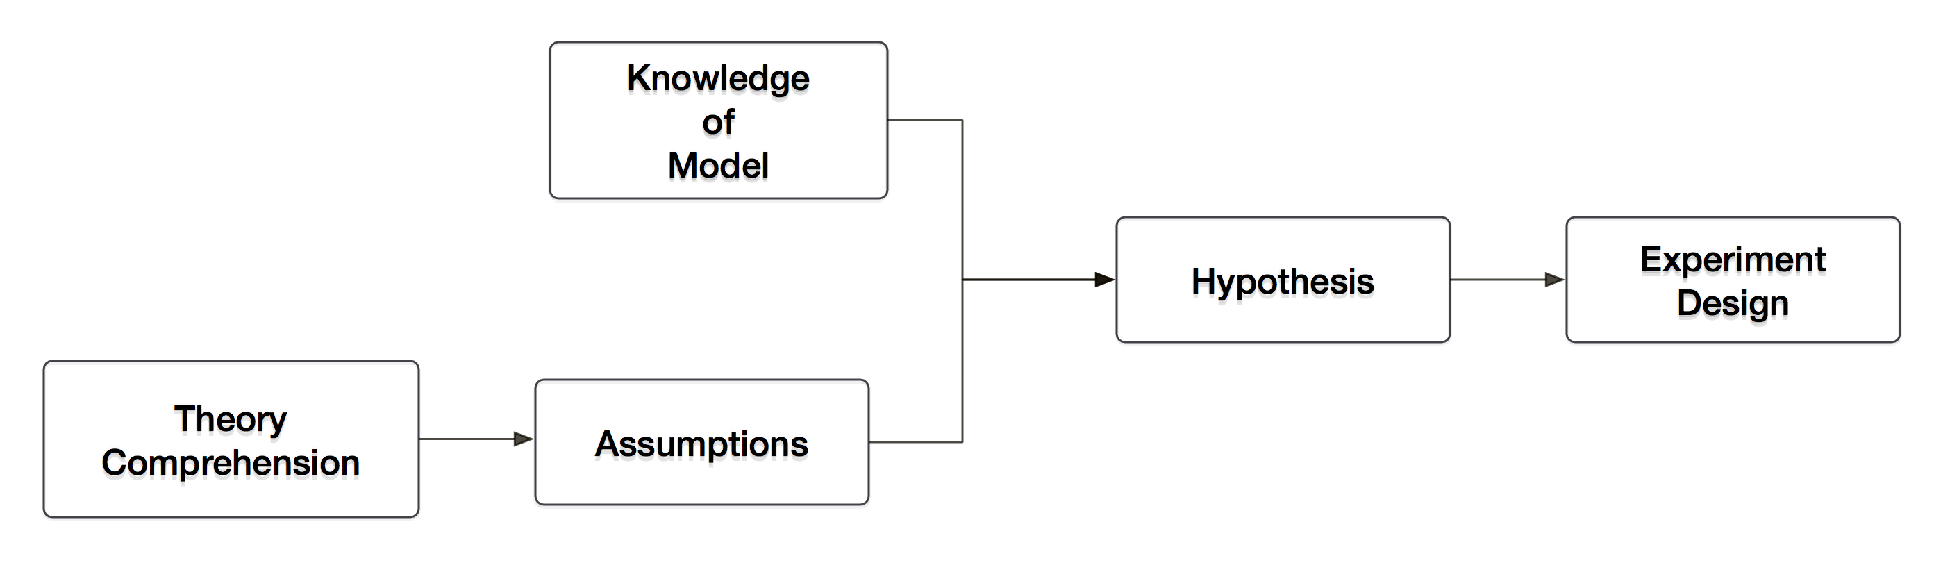
\includegraphics[width=\linewidth]{images/experiment-design}
	\caption{Traditional Experiment design workflow} 
  	\label{fig:experiment-design}
\end{figure}


From a theoretical point of view we decide to study RSP Engine facing their nature of linear dynamic system. Experiment design also require to point out which variable are observed, we simplify the study analysing their behaviour in term of Latency and Memory, as reported in Chapter \ref{chap:heaven}, and comparing the results of the four baselines (see Table \ref{tab:baselines-names}) in the experimental setting presented in the previous Section.

\subsection{SOAK: Tests and Hypothesis}\label{sec:soak-es}

Soak testing show the system dynamics, stressing the subject with a constant and continuous input flow, which in the Stream Reasoning context is the RDFStream. All the experiments are 20000 events long, this duration ensures the latency and the memory Steady State condition reaching for the majority of the experiment. Unlikely, is not possible to foretell how many events are required in to reach the Steady State condition for a certain variable. Multiple attempts and empirical evaluation are the only way to set up the correct longness. All experiment are executed 10 times, and we take the average to reduce measurement error. 

\begin{table}[htb]
\centering
 \begin{tabular}{l|c| lllll}
	  	\hline
		\multicolumn{2}{c|}{  } &\multicolumn{5}{c}{Window size}  \\
		\multicolumn{2}{c|}{  } & 1 & 10 & 100 &1000 &10000\\
		\hline
		\hline
		 & 1 & 1 & 10 & 100 & 1000&10000 \\
		\textsc{CTEvent}      & 10  & 10  & 100  & 1000 & 10000  \\
		size             &100   & 100   & 1000 & 10000  \\
					&1000   & 1000 & 10000 \\
					&10000   & 10000  \\
		\hline 
	\end{tabular}
	
	 \vspace{10pt}
	\caption{The number of triples in the window during the ten SOAK tests as a function of the Window size (in terms of $N$) and of the triples in each \textsc{CTEvent}.}
	\label{tab:soaktests}
\end{table}

Table \ref{tab:soaktests} presents the fifteen SOAK tests we run. for each baseline presented in Table \ref{tab:baselines-names}. The columns of the table are the different window sizes measured in terms of the values assumed by $N$.  Being $\beta=$ 100 ms., they  the corresponds to window that span 100 ms., 1 sec., 10 sec. and 100 sec.. The rows are the different number of triples in each CTEvent sent by the \textsc{RDF2RDF Streamer} to $\mathcal{E}$. Notably, for all of them, we checked that $\mathcal{E}$ is responsive for the whole duration of the experiment. 

The hypothesis to verify with SOAK experiments are:
\begin{itemize}
\item \textbf{HP.1} The Incremental reasoning approach is always better then the naive one.
\item \textbf{HP.2} The Graph-based model for RDFStream is always better then the Triple-based one.
\end{itemize}

\subsection{Step Response Tests}\label{sec:step-es}

Step Response testing allow to see how the system reacts to a sudden changing in the input condition. As we will see in the next section, SOAK tests show an initial warm-up phase for the system, with this set of experiment we can see if and how the warm-up changes is if we start from a stable running condition instead of starting from scratch.

We execute the step experiments concatenating two of the SOAK table, obtaining a total length of 400000 events, which means hours of execution for the system. For this reason we investigate only one window configuration, 10 slots window for all the four baselines. Table \ref{tab:steptests} summarises the experiment set-up,
\begin{table}[htb]
\centering
 \begin{tabular}{c|c|c}
	  	\hline
	  	&\multicolumn{2}{c}{CTEvent size}  \\
		Window Size & Initial Size & Final Size\\
		\hline
		\hline
		 10 & 10 & 100\\
		 10 & 10 & 1000\\
		 10 & 10 & 10000\\
		 10 & 100 & 1000\\
		 10 & 100 & 10000\\
		 10 & 1000 & 10000\\
		\hline 
 \end{tabular}
	\vspace{10pt}
 \caption{}
\label{tab:steptests}
\end{table}

The hypothesis to verify with Step experiments are:
\begin{itemize}
\item \textbf{HP.1} 
\item \textbf{HP.2}  one.
\end{itemize}

\subsection{Execution Environment}\label{sec:execution-environment}

All experiment are executed exploiting a dedicated machine, an iMac mid-2011 with 12GB RAM and 3.6 Ghz of a Intel i5 64 Bit, which run OS X 10.10.2 Yosemite,. Since \name is developed with Java 7\footnote{http://www.oracle.com/technetwork/java/javase/javase7locales-334809.html}, we use the versione 1.7.0.71 of the JVM.
The execution happens in a controlled environment, which tries to reduce the number of disturbing elements like network, graphical interface and other running processes.


\section{Evaluation Results}

The raw data results that comes of the experiment executions are in time series format, see Section \ref{sec:teststand} and in Section \ref{sec:teststand-impl} for details. Figure \ref{fig:data-processing} shows the phases which brings to the concrete analysis and the theoretic results. 

\begin{figure}[tbh]
  \centering
	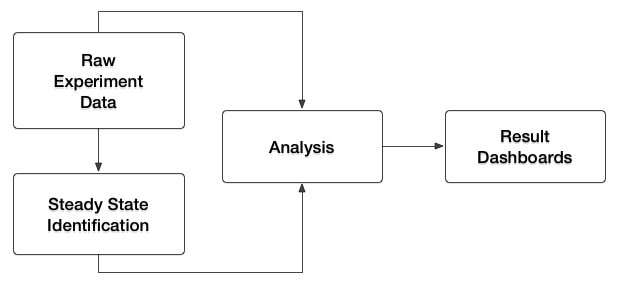
\includegraphics[width=\linewidth]{images/data-processing}
	\caption{From raw data processing to results dashboards} 
  	\label{fig:data-processing}
\end{figure}

We need the Steady State identification step because dynamic system usually has an initial warm-up phase which negatively influences results and inhibit generalisation and comparisons. To properly contrasts results between $n$ different RSP Engines data must be standardized. Automatic procedures to identify the State State condition exist, but requires dedicated studies which will be faced as future works. At this moment Steady State identification exploit data visualisation and is done by the researchers.  

Once the Steady State is identified we process all the data, weighting them w.r.t. the results of the Steady State post-processing analysis and the Hypothesis. Dashboards are the higher level of analysis offered by \namens. The Steady State data are presented in a n-dimension space which involves all the variables selected during the experiment design phase. Comparing solution trough dashboards it immediate, we can easily identify which solution, if any, is better then the other ones.




